\section{Тензор натяжений Максвелла. Давление магнитного поля.}

\begin{minipage}[c]{0.4\textwidth} % Левая часть: изображение
    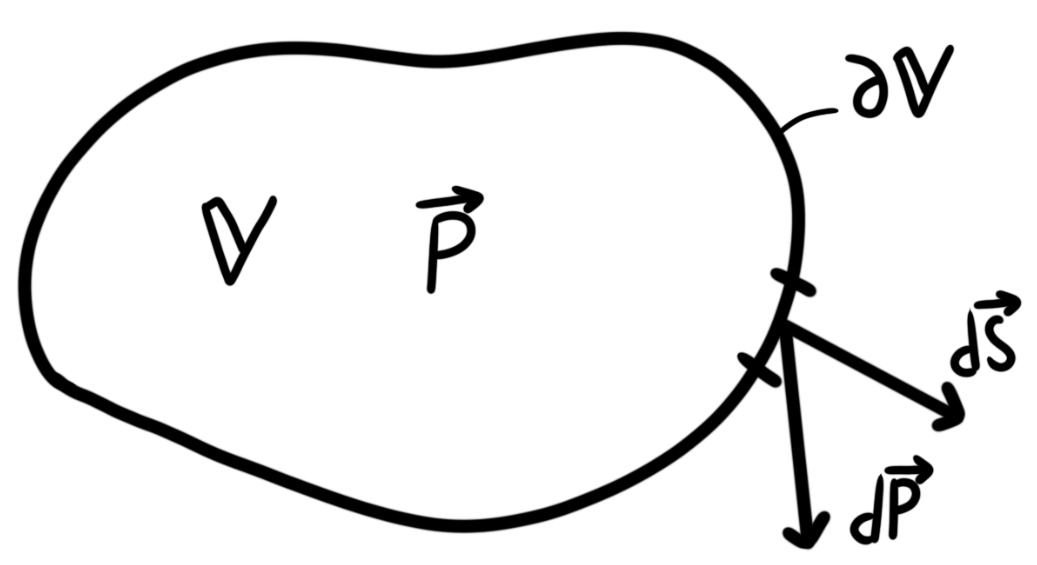
\includegraphics[width=\textwidth]{im/94.png}% Ваше изображение
\end{minipage}%
\hfill
\begin{minipage}[c]{0.6\textwidth} % Правая часть: текст
    \[
    \vec{P}=\underset{\mathbb{V}}{\iiint}=\vec{p}dV 
    \qquad 
    P_{\alpha}=\underset{\mathbb{V}}{\iiint}p_{\alpha}dV
    \]
\end{minipage}

\( \text{ } \) 

\[
\frac{\partial P_{\alpha}}{\partial t}=
\underset{\mathbb{V}}{\iiint} \frac{\partial p_{\alpha}}{\partial t}dV=
-\underset{\delta \mathbb{V}}{\oiint} \sigma_{\alpha\beta}dS_{\beta} \boxed{=}
\]

\begin{minipage}[c]{0.4\textwidth} % Левая часть: изображение
    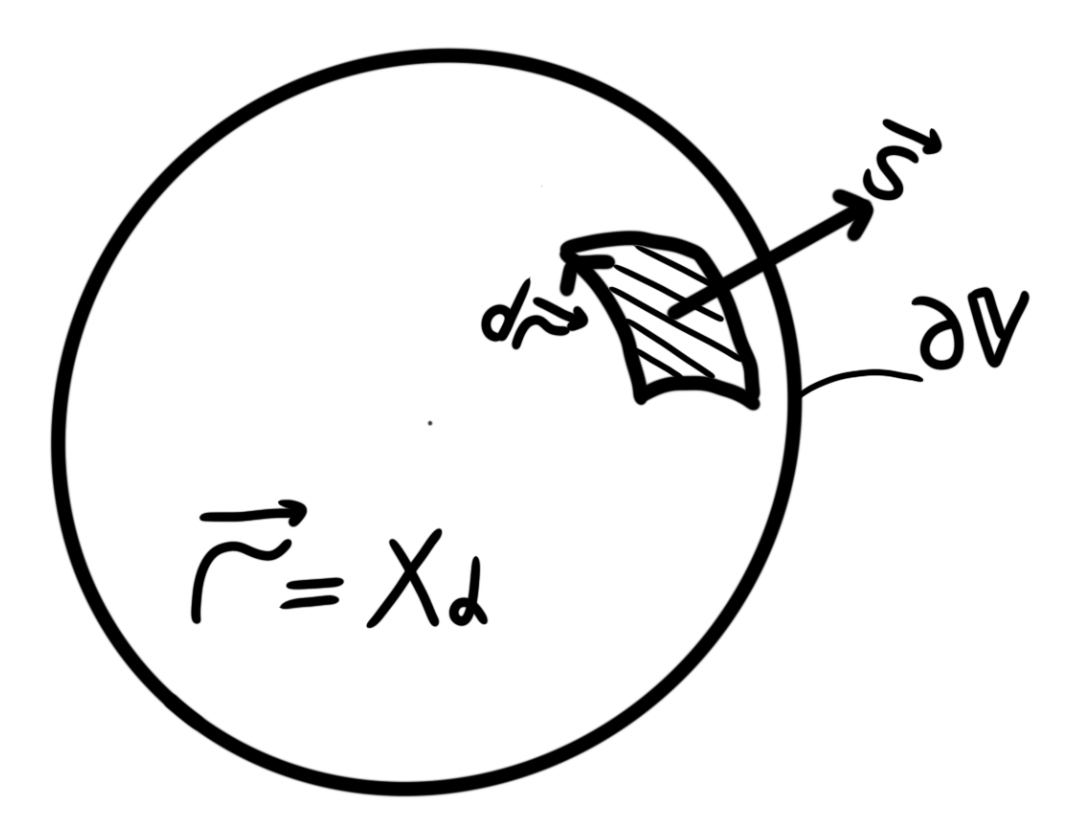
\includegraphics[width=\textwidth]{im/95.png}% Ваше изображение
\end{minipage}%
\hfill
\begin{minipage}[c]{0.6\textwidth} % Правая часть: текст
    \[
    dV=d\vec{r}d\vec{S}=d_{\alpha}dS_{\alpha}  
    \]
\end{minipage}

\begin{gather*}
    \boxed{=} -\underset{\mathbb{V}}{\iiint} \frac{\partial \sigma_{\alpha\beta} }{\partial x_{\beta} } \underbrace{dx_{\beta}dS_{\beta}}_{dV}=
    -\underset{\mathbb{V}}{\iiint}\frac{\partial \sigma_{\alpha\beta} }{\partial x_{\beta} }dV
\end{gather*}

Т.е нужно найти \( \sigma_{\alpha\beta}  \) такое, чтобы \( \frac{\partial P_{\alpha}}{\partial t}=-\frac{\partial \sigma_{\alpha\beta}}{\partial x_{\beta}}   \)

\begin{minipage}[c]{0.4\textwidth} % Левая часть: изображение
    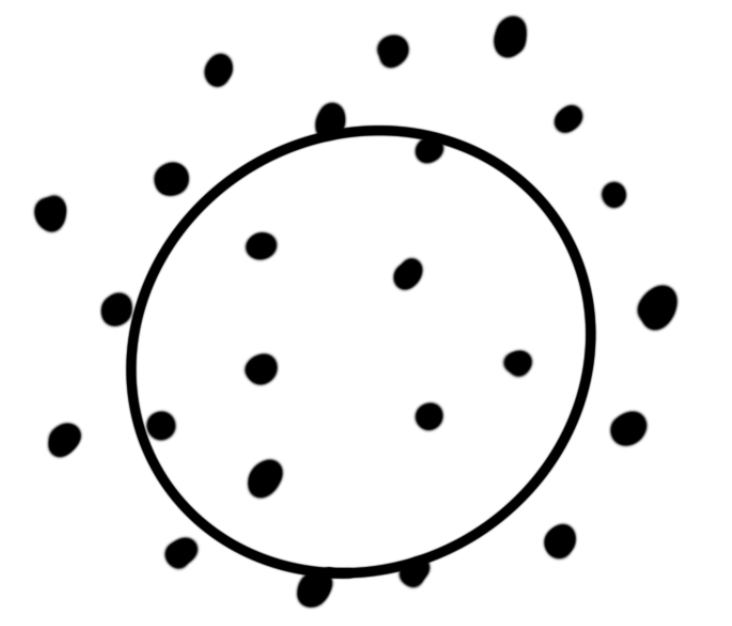
\includegraphics[width=\textwidth]{im/96.png}% Ваше изображение
\end{minipage}%
\hfill
\begin{minipage}[c]{0.6\textwidth} % Правая часть: текст
    \[
    \frac{d}{d t} (P_{r_{\alpha}}+P_{ n_{\alpha}})=-\frac{\partial \sigma_{\alpha\beta}}{\partial x_{\beta}}
    \]
    \( \qquad\qquad n \)- частицы
    
    \(\qquad\qquad r \)- поля 
\end{minipage}

\begin{gather*}
    \vec{F}=q\vec{E}+\frac{q}{c}[\vec{v}\times \vec{H}] \\
    \underset{\text{плотность силы}}{\vec{f}}=\vec{F}n=qn\vec{E}+\frac{1}{c}[\vec{j}\times \vec{H}] \\
    \frac{d\vec{P}_r}{dt}=\vec{f}=\rho\vec{E}+\frac{1}{c}[\vec{j}\times \vec{H}] 
\end{gather*}

Из выражений :

\begin{gather*}
    (\nabla \vec{E}) = 4\pi \rho  \\
    [\nabla \times \vec{ H}] = \frac{4\pi}{c} \vec{j} + \frac{1}{c} \frac{\partial \vec{E}}{\partial t} 
\end{gather*}

Следует:


\begin{gather*}
    \rho = \frac{1}{4\pi} (\nabla \vec{E})   \\
    \vec{j} = \frac{c}{4\pi} [\nabla \times \vec{H}] - \frac{1}{4\pi} \frac{\partial \vec{E}}{\partial t}
\end{gather*}

\begin{gather*}
    \frac{dP_{\alpha}}{dt}=\frac{1}{4\pi}\vec{E}(\grad\vec{E})+\frac{1}{4\pi}[[\grad \times  \overset{\downarrow}{\vec{H}}]\times \vec{H}]-\frac{1}{4\pi c} \left[ \frac{\partial \vec{E}}{\partial t} \times \vec{H} \right] = \\
    =\frac{1}{4\pi}\vec{E}[\grad\vec{E}]-\frac{1}{4\pi}\grad(\overset{\downarrow}{\vec{H}}\vec{H})+\frac{1}{4\pi}(\vec{H}\grad)\overset{\downarrow}{\vec{H}}-\frac{1}{4\pi c}\frac{\partial}{\partial t}[\vec{E}\times \vec{H}]+ \frac{1}{4\pi c} \left[ \vec{E}\times \frac{\partial\vec{H}}{\partial t}   \right]= \\
    =\frac{1}{4\pi}\vec{E}(\grad\vec{E})-\frac{1}{8\pi}\grad(H^2)+\frac{1}{4\pi}(\grad\overset{\downarrow}{\vec{H}})\overset{\downarrow}{\vec{H}}-\frac{1}{4\pi}\cancelto{0}{\vec{H}(\grad\overset{\downarrow}{\vec{H}})}-\frac{\partial}{\partial t}  \frac{\vec{S}}{c^2}+\frac{1}{4\pi}[\vec{E}\times [\grad \times \vec{E}]]= 
\end{gather*}

\begin{gather*}
    =\frac{1}{4\pi}[\vec{E}(\grad\vec{E})-\grad(\overset{\downarrow}{\vec{E}}+(\vec{E}\grad)\overset{\downarrow}{\vec{E}})]-\frac{1}{8\pi}\grad H^2 +\frac{1}{4\pi}(\grad \overset{\downarrow}{\vec{H}}) \overset{\downarrow}{\vec{H}} =\\
    =-\frac{1}{8\pi}\grad(E^2+H^2)+\frac{1}{4\pi}((\grad\overset{\downarrow}{\vec{E}})\vec{E}+(\grad\overset{\downarrow}{\vec{H}})\overset{\downarrow}{\vec{H}})- \frac{\partial}{\partial t} \frac{\vec{S} }{c^2}    
\end{gather*}

\[(\grad \vec{E})\vec{E}=\frac{\partial}{\partial x_{\beta} }E_{\beta}E_{\alpha}  \]

\begin{gather*}
    \frac{\partial}{\partial  t}(P_{r_{\alpha} }+P_{n_{\alpha} }  ) \quad \text{Тогда } \vec{P_n}=\frac{\vec{S}}{c^2}  \text{ и тогда:} \\
    \frac{\partial}{\partial  t}(P_{r_{\alpha} }+P_{n_{\alpha} }  )=-\left(\frac{\partial}{\partial x_{\alpha}}\left( \frac{1}{8\pi}(E^2+H^2)  \right) -\frac{1}{4\pi} \frac{\partial}{\partial  x_{\beta} (E_{\beta}E_{\alpha}+H_{\alpha}H_{\beta}    ) }      \right)= \\
    =-\frac{\partial}{\partial x_{\beta} } \left[ \underbrace{\frac{1}{8\pi}\delta_{\alpha\beta}(E^2+H^2)-\frac{1}{4\pi}(E_{\alpha}E_{\beta}+H_{\alpha}H_{\beta}  )   }_{\sigma_{\alpha\beta}} \right] 
\end{gather*}